\documentclass[9pt,twocolumn,twoside,lineno]{pnas-new}
% Use the lineno option to display guide line numbers if required.

\templatetype{pnasresearcharticle} % Choose template
% {pnasresearcharticle} = Template for a two-column research article
% {pnasmathematics} %= Template for a one-column mathematics article
% {pnasinvited} %= Template for a PNAS invited submission

% Math
\def\P{\mathbb{P}}
\def\cor{\mathrm{cor}}
\def\Quantile{\mathrm{Quantile}}
\def\logit{\mathrm{logit}}
\def\dist{\mathrm{dist}}
\def\WIS{\mathrm{WIS}}
\def\AUC{\mathrm{AUC}}
\newcommand{\indicator}[1]{\mathbf{1}\left(#1\right)}

% Figures and tables
\usepackage{xurl}
\usepackage{microtype}
\usepackage{booktabs}
\usepackage{caption}
\usepackage{subcaption}
\usepackage{xcolor}
\newcommand{\attn}[1]{\textcolor{red}{[ATTN: #1]}}

\makeatletter 
\renewcommand\@biblabel[1]{#1} 
\makeatother

% indicators
\newcommand{\chngcli}{CHNG-CLI}
\newcommand{\chngcov}{CHNG-COVID}
\newcommand{\dv}{DV-CLI}
\newcommand{\ar}{AR}
\newcommand{\fb}{CTIS-CLI-in-community}
\newcommand{\gs}{Google-AA}


\title{An Open Repository of Real-Time COVID-19 Indicators}

% Use letters for affiliations, numbers to show equal authorship (if applicable) and to indicate the corresponding author
\author[a,c,1]{Author One}
\author[b,1,2]{Author Two}
\author[a]{Author Three}

\affil[a]{Affiliation One}
\affil[b]{Affiliation Two}
\affil[c]{Affiliation Three}

% Please give the surname of the lead author for the running footer
\leadauthor{Lead author last name}

% Please add a significance statement to explain the relevance of your work
\significancestatement{To study the COVID-19 pandemic, its effects on society,
  and measures for reducing its spread, researchers need detailed data on the
  course of the pandemic. Standard public health data streams suffer
  inconsistent reporting and frequent, unexpected revisions. They also miss
  other aspects of a population's behavior, worthy of consideration. We
  present an open database of COVID signals in the United States, measured at
  the county level and updated daily. These include traditionally reported COVID
  cases and deaths, and many others: signals based on measures of mobility,
  social distancing, internet search trends, self-reported symptoms, and
  patterns COVID-related activity in de-identified medical insurance claims. The
  database provides all signals in a common, easy-to-use format, empowering both
  public health research and operational decision-making.
}

% Please include corresponding author, author contribution and author declaration information
\authorcontributions{Please provide details of author contributions here.}
\authordeclaration{Please declare any competing interests here.}
\equalauthors{\textsuperscript{1}A.O.(Author One) contributed equally to this work with A.T. (Author Two) (remove if not applicable).}
\correspondingauthor{\textsuperscript{2}To whom correspondence should be addressed. E-mail: author.two\@email.com}

% At least three keywords are required at submission. Please provide three to five keywords, separated by the pipe symbol.
\keywords{open data $|$ COVID-19 $|$ digital surveillance $|$ medical insurance
  claims $|$ internet surveys $|$ search trends $|$ mobility patterns}

\begin{abstract}
  Please provide an abstract of no more than 250 words in a single paragraph.
  Abstracts should explain to the general reader the major contributions of the
  article. References in the abstract must be cited in full within the abstract
  itself and cited in the text.
\end{abstract}

\dates{This manuscript was compiled on \today}
\doi{\url{www.pnas.org/cgi/doi/10.1073/pnas.XXXXXXXXXX}}

\begin{document}

\maketitle
\thispagestyle{firststyle}
\ifthenelse{\boolean{shortarticle}}{\ifthenelse{\boolean{singlecolumn}}{\abscontentformatted}{\abscontent}}{}

\dropcap{P}ublic health decision-makers, healthcare providers, epidemiological
researchers, employers, institutions, and the general public benefit from
promptly and readily accessible data regarding COVID-19 activity levels,
countermeasures, and pandemic impact.  Real-time indicators of COVID-19 activity
levels, such as statistics on cases, deaths, test positivity, and
hospitalizations, enable reports and interactive dashboard applications for
situational awareness \cite{Dong:2020, NYTimes, USAFacts}, and are essential for
most analyses of the pandemic.  These data are available for locations across
the United States from a number of official sources and independent aggregators
in varied and inconsistent formats.  Different data types and sources vary in
timeliness, based on when measured events occur in the progression of the
disease, testing capabilities, the reporting pipeline, and their publication
schedules.

Additional, auxiliary data sources can improve on the timeliness, scope, and
utility of the ``topline'' indicators (cases, test positivity, hospitalizations,
deaths) coming from the public health reporting system. For example, in the
context of other infectious diseases: syndromic surveillance in ambulatory
clinics and emergency rooms improves the accuracy of outbreak detection for
emerging pathogens such as H1N1 \cite{Kass-Hout:2012}; and digital surveillance
(based on, e.g., search and social media trends) enable more accurate
``nowcasts'' and forecasts of traditional disease surveillance streams such as
the CDC's ILINet \cite{Santillana:2015, Farrow:2016}, as do publication formats
providing access to historical versions of a data set \cite{Brooks:2018,
  Brooks:2020}. Numerous other examples exist spanning a wide variety of data
platforms and diseases \cite{Browstein:2009, Kass-Hout:2011, Salathe:2012,
  Kass-Hout:2013}. During the COVID-19 pandemic, digital data streams have
permitted faster prediction of case increases \cite{Ahmad:2020, Kogan:2021},
while enabling analyses of the impact of public health policies on public
behavior, the economy, and disease spread \cite{Bonaccorsi:2020, Nouvellet:2021,
  Adjodah:2021, Jewell:2021}.

The Delphi Group works with partner organizations and public data sets to build
a massive database of indicators tracking COVID-19 activity and other relevant
phenomena, which has been publicly available and continuously updated since
April 2020. Alongside public data on reported cases and deaths, this database
includes several unique data streams, including indicators extracted from
de-identified medical claims data, antigen test results from a major testing
manufacturer, large-scale public surveys that measure symptoms and public
behavior, and symptom indicators based on Google search query volume. (We use
the terms ``indicator'' and ``signal'' interchangeably.) We make aggregate
signals publicly available, generally at the county level, via the COVIDcast API  
\cite{CovidcastAPI}. We store and provide access to all previous (historical)
versions of the signals, a key feature that exposes the effects of data
revisions.  Lastly, we provide R \cite{CovidcastR} and Python \cite{CovidcastPy}  
packages to facilitate interaction with the API, and an online dashboard to
visualize the data \cite{CovidcastViz}. 

% RJT: We should fiddle with the bib so that the URLs actually appear in the
% references at the end.  Otherwise it's kind of pointless to cite manuals or
% websites like the COVIDcast API site or R/Python manuals.

In a companion paper, we analyze the utility provided by a core set of the
indicators in COVID-19 forecasting and hotspot prediction models.  In another
companion paper, we elaborate on our research group's (Delphi's) large-scale
public surveys, run in partnership with Facebook and available in aggregate form
in the COVIDcast API.

\section{Methods}

\subsection{Data Collection}

We receive data daily from healthcare partners, technology companies, and from
surveys conducted daily by Delphi in partnership with Facebook. These data
sources provide information not available from standard public health reporting
or other common sources, such as:
\begin{description}
\item[Health Insurance Claims] Based on de-identified medical insurance claims
  from Change Healthcare and other health system partners, we release indicators
  on the estimated percentage of covered outpatient visits and hospitalizations
  that involved COVID diagnoses or symptoms.
\item[Internet-Based Surveys] Conducted in partnership with Facebook, Delphi's
  COVID Tracking and Impact Survey receives about 50,000 responses daily, and
  has received over 20 million responses since April 2020 \cite{DelphiSurvey,
    Kreuter:2020}. From the surveys, we construct indicators on symptoms,
  social distancing, vaccination, and other attitudes and behaviors related to
  COVID.
\item[COVID Antigen Tests] Based on data from Quidel, a major manufacturer of
  COVID antigen tests in the United States, we calculate and release
  (Quidel-specific) test volumes and positivity rates.
\item[Search Trends] Based on Google's COVID-19 Search Trends symptoms data set
  \cite{GoogleSymptoms}, we provide indicators reflecting COVID-related search
  activity.
\item[Mobility Data] Cell phone mobility data is collected by SafeGraph
  \cite{SafeGraphSD, SafeGraphPatterns}, and is available to researchers under a
  data use agreement; we aggregate it to the county level and make indicators
  publicly available.
\end{description}

We also scrape data accessible from other public sources, such as cases and
deaths data aggregated from public reporting by JHU CSSE \cite{Dong:2020} and by
USAFacts \cite{USAFacts}, so that we can track revisions and updates to this data
(see Section~\ref{subsec:revision_tracking}).

Together, we collect TODO signals from TODO distinct sources, aggregate them,
and provide them in a single common format for public access. This hence
provides a common format both for unique data streams not available elsewhere
and for public data streams, enabling efficient comparison and modeling use.

A summary of the data sources we currently receive and make available is
presented in Table~\ref{data-sources}, and detailed documentation of the signals
available from each source is available at
\url{https://cmu-delphi.github.io/delphi-epidata/api/covidcast_signals.html}.

\begin{table*}
\centering
\caption{Data sources available in Delphi's COVIDcast API \cite{CovidcastAPI},
  as of date of publication. The first group of data sources are produced by
  Delphi from data not otherwise available publicly (or only available in
  limited form); the second group is mirrored from public sources.}
\begin{tabular}{>{\raggedright}p{1.2in} p{4.0in} r >{\raggedright\arraybackslash}p{0.5in}}\toprule
\textbf{Data source} & \textbf{Signals available} & \textbf{First date} &
\textbf{Resolution} \\\midrule
  % Exclusive data
  Change Healthcare & Percentage of outpatient visits with COVID diagnostic codes
or codes indicating COVID-like symptoms. Based on de-identified claims data
processed by Change Healthcare. & 2020-02-01 & County$^*$ \\
  Doctor Visits & Percentage of outpatient visits primarily about COVID-like
symptoms, based on de-identified claims data provided by health system
partners. & 2020-02-01 & County$^*$ \\
  Hospital Admissions & Percentage of new hospital admissions with COVID
diagnostic codes, based on de-identified claims data provided by health system
partners. & 2020-02-01 & County$^{**}$\\
  Quidel & Test positivity rates for COVID-19 antigen tests produced by
Quidel. & 2020-05-26 & County$^{**}$ \\
  SafeGraph & Mobility metrics, such as time away from home or visits to bars
and restaurants, based on cell phone mobility data collected by SafeGraph
\cite{SafeGraphSD, SafeGraphPatterns}. & 2019-01-01 & County \\
 COVID Tracking and Impact Survey & COVID symptoms, social distancing behaviors,
mental health, economic impact, behavior (e.g., mask-wearing, vaccination
attitudes), and COVID testing signals based on daily surveys conducted
nationally by Delphi through Facebook \cite{DelphiSurvey, Kreuter:2020}. &
2020-04-06 & County$^{**}$ \\
  \midrule
    % Mirrored data from other sources
  Health \& Human Services & Counts of hospital admissions due to confirmed or
suspected COVID-19, as reported by the Department of Health \& Human Services. &
2019-12-31 & State \\
    COVID Act Now & COVID-19 testing results, such as positivity and number of
tests, compiled by COVID Act Now from CDC reporting. & 2020-03-02 &
County$^*$ \\
  Google Symptoms & Trends in Google search volume for terms related to anosmia
and ageusia (loss of smell or taste), which correlate with COVID activity, based
on data shared by Google \cite{GoogleSymptoms}. & 2020-02-13 & County$^{***}$ \\
  Cases and Deaths & Confirmed COVID-19 cases and deaths, compiled by JHU CSSE
\cite{Dong:2020} and by USAFacts \cite{USAFacts}. & 2020-01-22 & County \\
  NCHS Mortality & Weekly totals of deaths broken down by cause, such as COVID,
flu, or pneumonia, compiled by the National Center for Health Statistics [TODO
cite]. & 2020-01-26 & State \\
    \bottomrule
\end{tabular}
% TODO PNAS wants a short title above and caption below, but they can't possibly
% mean for the caption to be formatted so weirdly...
\addtabletext{Location availability often drops lower for some times and
  signals, e.g., due to variable reporting volume. $^*$Available at $>60$\% of
  counties; $^{**}$available at 20--60\% of counties; $^{***}$available at
  $<20$\% of counties.}
\label{data-sources}
\end{table*}

\subsection{Signal Processing}

Because each data source reports data in different formats, we must convert each
source to a common format. In this format, each record represents an observation
of one quantity at one time point in one location. Locations are coded
consistently using standard identifiers such as FIPS codes; the sample size and
standard error for each observation is also reported when applicable. Each
signal is reported at the finest geographic resolution its source supports (such
as county or state) and also aggregated to metropolitan statistical areas,
Health and Human Services regions, and Hospital Referral Regions. National
averages are also provided. Crucially, each record includes an \textit{issue
  date} recording when the value was first issued, as described below. This
allows tracking of multiple revisions to individual observations, each revision
with a separate issue date.

When appropriate, additional post-processing (often nontrivial) is applied to
the data. For example, data on visits to doctor's offices is subject to strong
day-of-week effects, and so regression is used to adjust for these
effects. Other indicators are available in raw versions and versions smoothed
with a seven-day moving average. All processing is done using open-source code
written primarily in Python and R, and available publicly at
\url{https://github.com/cmu-delphi/covidcast-indicators/}.

\subsection{Revision Tracking}
\label{subsec:revision_tracking}

Many data sources that are useful for epidemic tracking are subject to revision
after their initial publication. For example, aggregated medical claims data may
be initially published after several days, but additional claims and corrections
may take days to weeks to be discovered, processed, and aggregated. Medical
testing data are also often subject to backlogs and reporting delays, and
estimates for any particular date are revised over time as errors are found or
additional data becomes available. This revision process is generally referred
to as \textit{backfill}.

For this reason, the COVIDcast API annotates every observation with two dates:
the \textit{time value}, the date the underlying events (such as tests or
doctor's visits) occurred, and the \textit{issue date} when Delphi aggregated
and reported the data for that time value. Importantly, there can be multiple
observations for a single time value with different issue dates, for example if
data is revised or claims records arrive late. Delphi tracks revisions to all
data sources we ingest, including external data sources (such as sources
tracking cases and deaths). Many external sources do not keep a public or
conveniently accessible record of revisions of their data.

For many purposes it is sufficient to use the most recently issued observation
for any time value, and thus the COVIDcast API reports the most recent issue by
default. However, for some applications it is crucial to know what was known
\textit{as of} a specific date. For example, an epidemic forecasting model will
be called upon to make its forecasts based on preliminary data about recent
trends, and so when it is trained using historical data, it should be trained
using the initial versions of that data, not updates that would have been
received later. Furthermore, these revision records allow models to be modified
to account for noise and bias in early data versions, or to exclude data that is
too new to be considered stable, and to ``rewind'' time and simulate how these
revised models would have performed using only the versions of data available
\textit{as of} those times.

Research on data revisions in the context of influenza-like illness has shown
that backfill can significantly alter forecast performance \cite{Brooks:2018,
  Reich:2019}, and that training to use preliminary data can reduce this
influence \cite{Brooks:2018, Brooks:2020}. This is also investigated in our
companion paper on forecasting, where we observe that training and validating
models on finalized data yields overly optimistic estimates of true test-time
performance.  

\subsection{Public API}

The data described above is publicly available through the Delphi COVIDcast API
\cite{CovidcastAPI}.  By making HTTP requests specifying the data source,
signal, geographic level, and time period desired, users can receive data in
JSON or CSV form. For added convenience, we have written \texttt{covidcast} R
\cite{CovidcastR} and Python \cite{CovidcastPy} packages with functions to
request data, format it as a data frame, plot and map it, and combine it with
data from other sources.

The R and Python package software is public and open-source, at
\url{https://github.com/cmu-delphi/covidcast/}.  The underlying server software
is itself also public and open-source, at
\url{https://github.com/cmu-delphi/delphi-epidata/}.  Lastly, most data sources
are provided under the Creative Commons Attribution license, and a small number
have additional restrictions imposed by the data source; see
\url{https://cmu-delphi.github.io/delphi-epidata/api/covidcast_licensing.html}.

\subsection{Interactive Visualization}

% RJT: @AR I'm now thinking we should add a very short paragraph or two on
% this. We can say that we provide various interactive maps highlighting both
% temporal (time series) and spatial aspects (choropleth or beehive maps), but
% also exploratory tools for correlations and anomalies.  (Very much like the
% correlations computed in the next section.)

% Another reason why I'm in favor of this is that we can now add everybody as a
% middle author who now contributed anything at all to COVIDcast, from database
% to API to indicator to visualization.  I'm sure the HCII students & faculty
% who worked with us would very much appreciate being on this paper.

\section{Results}

The indicators that are available in the COVIDcast API have been used in
dashboards produced by COVID Act Now \cite{CovidActNow}, COVID Exit Strategy
\cite{CovidExitStrategy}, and others; to inform the Delphi, DeepCOVID
\cite{Rodriguez:2021}, and the Institute for Health Metrics and Evaluation
(IHME) \cite{IHMEProj} COVID forecasting models; in various federal and state
government reports and analyses; and in a range of news stories. Aside from
operational use in decision-making and forecasting, they have also facilitated
numerous analyses studying the impacts of COVID-19 on the public, the
effectiveness of policy interventions, and factors that influenced the spread of
the pandemic \cite{Adjodah:2021, Pierri:2021, Jewell:2021, Chakrabarti:2020,
  Doerr:2021}. The API currently serves hundreds of thousands of requests each
day, to thousands of users worldwide.

In what follows, we present illustrative examples of the usefulness of some of
the novel signals available in the API. These examples demonstrate that such
indicators are meaningfully related to COVID activity, that they provide
alternate views on pandemic activity that are not subject to the same reporting
glitches and delays as traditional public health surveillance streams, and that
they provide information about public behavior and attitudes that are not
available from any other source. Code to reproduce all examples (which uses the
\texttt{covidcast} R package and fetches data directly from the API) can be
found at \url{TODO}.

\subsection{Tracking Trends}

\begin{figure}
  \centering
  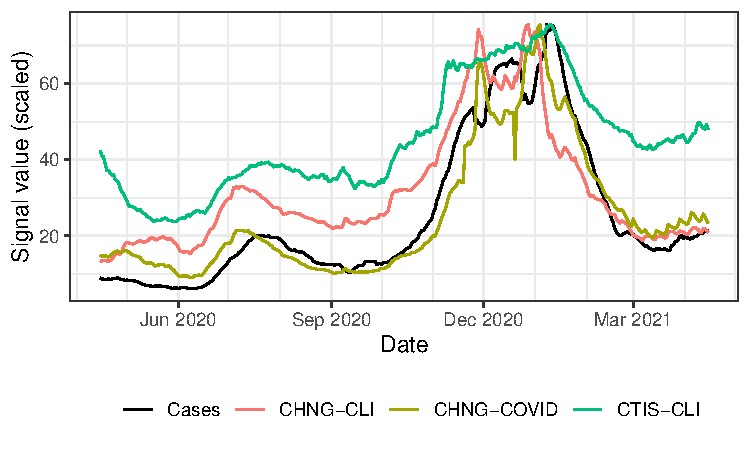
\includegraphics[width=\columnwidth]{fig/time_trends_national.pdf}
  \caption{National trends, from April 2020 to April 2021, of four signals in
    the COVIDcast API. The auxiliary signals, based on medical claims data and
    massive surveys, track changes in officially reported cases quite
    well. (They have all been placed on the same scale as reported cases per
    100,000 people.)}
  \label{fig:time_trends_national}
\end{figure}

Many of the indicators in the COVIDcast API are intended to track COVID
activity. Five indicators in particular have the closest connections to
confirmed COVID cases:
\begin{itemize}
\item Change Healthcare COVID-like illness (CHNG-CLI): The percentage of
  outpatient visits that are primarily about COVID-related symptoms, based on
  de-identified Change Healthcare claims data.
\item Change Healthcare COVID (CHNG-COVID): The percentage of outpatient visits
  with confirmed COVID-19, based on the same claims data.
\item COVID Tracking and Impact Survey CLI (CTIS-CLI): The estimated percentage
  of the population with COVID-like illness based on Delphi's surveys of
  Facebook users.
\item COVID Tracking and Impact Survey CLI-in-community (CTIS-CLI-in-community):
  The estimated percentage of the population who knows someone who is sick,
  based on Delphi's surveys of Facebook users.
\item Quidel COVID test positivity rate (Quidel-TPR): The percentage of positive
  test results among Quidel COVID antigen tests.
\end{itemize}
Figure~\ref{fig:time_trends_national} compares the first three of these signals
to reported COVID cases in the United States (from JHU CSSE, and smoothed with a
7-day trailing average) over the first year of the pandemic (April 15, 2020 to
April 15, 2021), illustrating how they  appear to track national trends in cases
quite well. Importantly, this same relationship persists broadly across multiple
resolutions, down to smaller geographic regions such as states and counties, as
shown in the supplement. This will also be illustrated in a more detailed
correlation analysis in the next subsection.

% RJT: @AR Note what I claimed we would do above!  I'm thinking we can just
% produce a big batch of case trends over the same time period and for the same
% signals, but for each US state (and territory?), and for the 50 most populous
% counties. AND maybe for this (below national) we should use CLI-in-community
% rather than CLI, from the survey

Besides tracking contemporaneous COVID activity, these and other indicators can
be used to improve forecasts of future COVID case trends, as investigated in a
companion paper.

% RJT: @AR Consider for the supplement.
% - Hospitalization trends?
% - Hospitalization correlations?
%  (I see you already have a plot for the first ... but I'm a bit bothered by
%  the fact that the HHS data looks to have such strong weekday effects that we
%  don't attempt to correct for ... perhaps we use do a 7-day rolling avg. Made
%  easy with modeltools)
% If we do so, we should refer to it in the text, this subsection (for time
% trends) and next (for correlations)

\subsection{Correlation Analyses}

To quantify the ability of the signals described above to track trends in COVID
cases, we use the Spearman (rank) correlation and analyze two key correlation
patterns, between each signal and confirmed COVID case rates (cases per 100,000
people):
\begin{enumerate}
\item \textit{Geo-wise correlations} (i.e., on a specific date, do values of the
  signal correlate with case rates across locations?): Formally, let $X_t$ and
  $Y_t$ be vectors of values of a particular signal and case rates, over all
  locations, on date $t$. The geo-wise correlation at time $t$ is defined as
  $\cor(X_t, Y_t)$. This examines whether a signal has the capability to help
  spot locations with high case rates at any given time.

\item \textit{Time-wise correlations} (i.e., at a specific location, do values
  of the signal correlate with case rates across time?): Formally, let $X_\ell$
  and $Y_\ell$ be vectors of a values of a particular signal and case rates,
  over all times, at location $\ell$. The time-wise correlation at time $t$ is
  defined as $\cor(X_\ell, Y_\ell)$. This examines whether changes in a signal
  over time correspond to changes in reported cases at the same location.
\end{enumerate}

\begin{figure}[t]

  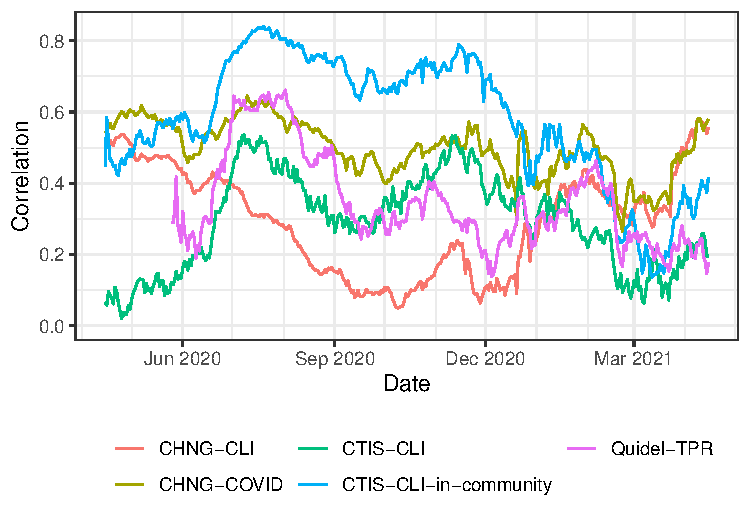
\includegraphics[width=\columnwidth]{fig/geo_wise_corr.pdf}
  \caption{Geo-wise correlations with case rates, from April 15, 2020 to April
    15, 2021, calculated over all counties for which all signals were available
    and which had at least 500 cumulative cases by the end of this period.}
 \label{fig:geo_wise_correlation}
\end{figure}

Figure~\ref{fig:geo_wise_correlation} shows the geo-wise correlations achieved
by the five signals and COVID case rates (from USAFacts, and again smoothed
using a 7-day trailing average), from April 15, 2020 to April 15, 2021. The
locations we consider here are counties with at least 500 cumulative cases by
the end of this period, and at which all signals are available (956 counties in
total). The  significantly positive correlations suggest that these signals
could be useful in hotspot detection  (identifying counties with relatively high
COVID activity, at a given time). Somewhat surprisingly, the CLI-in-community
signal derived from the survey shows the strongest correlations for much of the
time period. This clearly demonstrates the value of a large-scale survey such as
CTIS for tracking symptoms and case trends, especially when other data is
unavailable.

Figure~\ref{fig:time_wise_correlation} summarizes time-wise correlations of
these five signals over the same time period, and for the same set of
counties. For each signal, we display the set correlations that it achieves in
histogram form (more precisely, using a kernel density estimate). All signals
produce positive correlations in the majority of counties considered (with very
little mass in each estimated density being to the left of zero). The largest
correlations, in bulk, are achieved by the CHNG-COVID signal; the
CTIS-CLI-in-community is a close second, and the CHNG-CLI signal is third.
There are two remarks deserving attention:

\begin{figure}[t]
  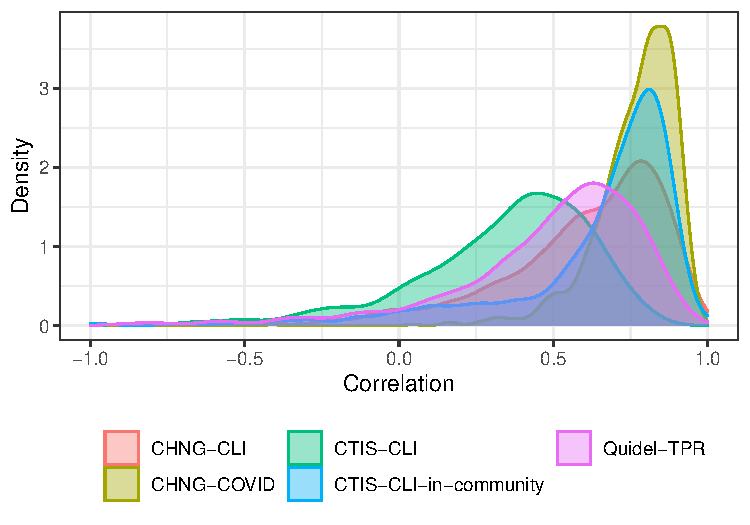
\includegraphics[width=\columnwidth]{fig/time_wise_correlation.pdf}
  \caption{Time-wise correlations with case rates, from April 15, 2020 to April
    15, 2021, calculated over all counties for which all signals were available
    and which had at least 500 cumulative cases by the end of this period.}
  \label{fig:time_wise_correlation}
 \end{figure}

\begin{itemize}
\item This is different from what is observed in
  Figure~\ref{fig:geo_wise_correlation}, where the CTIS-CLI-in-community signal
  achieves clearly the highest correlations for most of the time
  period. However, it is worth emphasizing that time-wise and geo-wise
  correlations are truly measuring different properties of a signal; and the
  claims signals (CHNG-COVID and CHNG-CLI) seem more appropriate for
  temporal---rather than spatial---comparisons.  We revisit this point in the
  discussion.
\item It is still quite impressive and surprising that the CTIS-CLI-in-community
  signal, based on people reporting on the symptoms of others around them, can
  achieve  nearly as strong time-wise correlations to confirmed cases as can a
  signal that is based on picking up the occurrence of a confirmed case passing
  through the outpatient system.
\end{itemize}

\subsection{Helping Robustness}

Public health reporting of COVID tests, cases, deaths, and hospitalizations is
subject to a number of possible delays and problems. For example, COVID testing
data is reported inconsistently by different states using different definitions
and inclusion criteria, and differences in reporting processes mean state data
often does not match data reported to the federal government
\cite{Schechtman:2021}. Case and death data is frequently backlogged and
corrected, resulting in artificial spikes and drops \cite{Simon:2021,
  ArvisaisAnhalt:2021}.

As an example, looking back at Figure \ref{fig:time_trends_national}, we can see
clear dips in the confirmed COVID case curve that occur around the Thanksgiving
and New Year's holidays. This is artificial, and due to the fact that public
health departments usually close over holiday periods, which delays case and
death reporting (for this reason, the artificial dips persist at the state- and
county-level as well). The CLI signal from the survey, on the other hand,
displays no such dips. The claims signals actually display holiday effects going
in the other direction: they exhibit \textit{spikes} around Thanksgiving and New
Year's. This is because they measure the fraction of all outpatient visits with
a certain condition, and the denominator here (total outpatient visits) drops
disproportionately during holiday periods, as people are likely less willing to
go to the doctor for more routine issues. Fortunately, in principle, the holiday
effects in claims signals should be correctable: they are mainly due to
\textit{overall} changes in medical seeking behavior during holiday, periods,
and we can estimate such effects using historical claims data.

As a further example, Figure~\ref{fig:bexar-compare} displays data from Bexar
County, Texas (which contains San Antonio) during July 2020. On July 16, 2020,
4,810 backlogged cases were reported after reporting problems prevented them
from being reported over the past two weeks \cite{Palacios:2021}. This results
in a clearly visible spike in the left-hand panel of the figure (case data from
JHU CSSE, smoothed with a 7-day trailing average).  However, Delphi's COVID
Tracking and Impact Survey averaged around 350 responses per day in Bexar
County over the same time period, and was able to estimate the fraction
of the population who know someone in their community with COVID-Like Illness
(CLI). As we can see in the right-hand panel of the figure, this signal was not
affected by Bexar County's reporting problems and, as shown in the last
subsection, it is (in general) highly correlated with case rates, providing an
alternate stream of data about COVID activity unaffected by backlogs. Similar
reporting problems have occurred in many jurisdictions across the United States,
making it valuable to cross-check against external sources not part of the same
reporting systems.

\begin{figure}
  \centering
  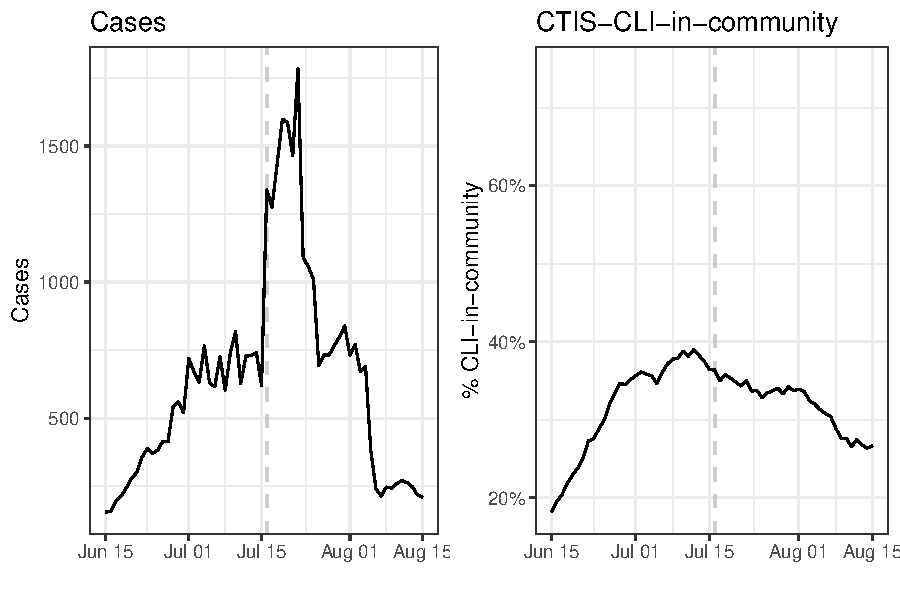
\includegraphics[width=\columnwidth]{fig/bexar_compare.pdf}
  \caption{Reported cases per day in Bexar County, Texas during the summer of
    2020. Only July 16, 4,810 backlogged cases were reported, though they
    actually occurred over the preceding two weeks (this shows up as a prolonged
    spike in the left panel due to the 7-day trailing averaging applied to the
    case counts). Daily CTIS estimates of CLI-in-community showed more stable
    underlying trends.}
  \label{fig:bexar-compare}
\end{figure}

\subsection{Revisions Matter}

The revision tracking feature in the API assists in model-building and
evaluation. Figure~\ref{fig:dv_as_of} illustrates how one COVIDcast medical
claims signal evolved as it was revised across multiple issue dates, in four
different states, between June 1 and August 1, 2020. In each plot, the rightmost
ends of the lines correspond to estimates for the last day that data are
available for each issue date, which are generally the most tentative estimates,
and appear to be significantly biased upward in Arizona in June 2020, and
significantly biased downward in New York throughout June and July 2020.

\begin{figure}
\centering
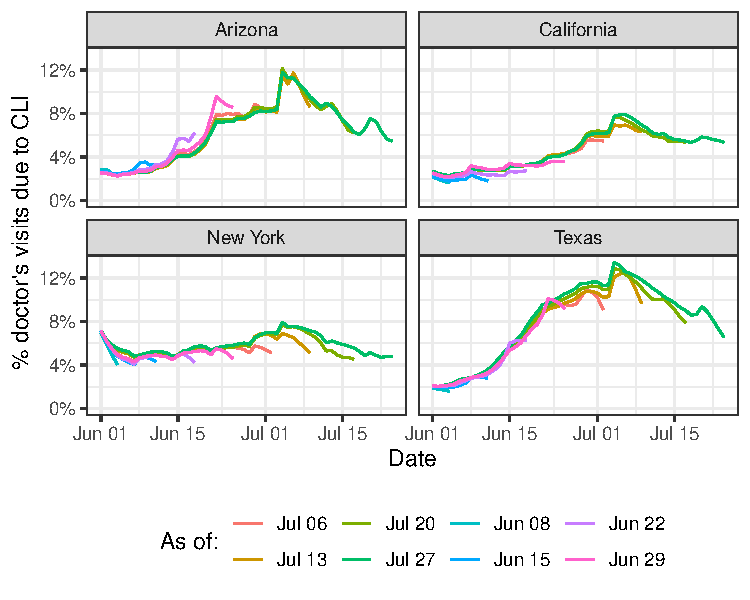
\includegraphics[width=\columnwidth]{fig/dv_as_of.pdf}
\caption{Estimated percentage of doctor's visits due to COVID-like illness
  displayed across multiple issue dates, with later issue dates adding
  additional data and revising past data from prior issue dates.}
\label{fig:dv_as_of}
\end{figure}

Claims-based signals typically undergo heavy backfill as additional claims are
processed and errors are corrected; the median relative error between initial
reports and final values is over 20\% for such data, and only after roughly 35
days do estimates typically match finalized values within 5\%. However, the
systematic nature of this backfill, as illustrated in Figure~\ref{fig:dv_as_of},
suggests that statistical models could be fit (potentially separately for each
location) to estimate the final values from preliminary reports. On the other
hand, official public health reporting of COVID cases and deaths can be subject
to revision as death certificates are audited and backlogs cleared, resulting in
thousands of cases and deaths being added or removed. This process is much more
difficult to predict, and thus claims data and other sources may be a useful
stand-in while public health reports are aggregated and corrected.

To reiterate a previous point, when training and validating forecast models (on
historical data), users will want to use data that was known \textit{as of} the
forecast date, not revised versions that only became available much later. The
COVIDcast API makes all historical versions available and easily accessible for
this purpose; and this feature plays a prominent role in our own analysis of
forecasting and hotspot prediction models appearing in a companion paper.

\subsection{New Perspectives}

Auxiliary signals (outside of the standard public health reporting streams) can
serve as indicators of COVID activity, but they can also illuminate other
aspects of the pandemic. To understand the effect of the pandemic on society and
predict its future spread requires a comprehensive view of not just cases and
deaths, but public behavior and beliefs. Measures of mobility reflect social
distancing policies and the potential rate of COVID spread; medical claims data
reflects healthcare-seeking behavior and how it may be affected by local case
rates; measures of COVID vaccine acceptance can guide outreach efforts
\cite{TODO}.

% AR: Potentially interesting things to show or comment on:
% - Medical claims data can give info about medical-seeking behavior and how it
% varies with caseload -- e.g. are people deterred from seeking medical care
% because of the high case load?
% - Mobility changes
% - Map of one of the unique signals during an outbreak, e.g. Michigan in April
% 2021

% RJT: @AR Since we already stuff on claims, can we do: mobility, masks, vaccine
% uptake or hesitancy, distancing behaviors, how worried are you?

% How about this (in each case, each point in said plot is a county's signal
% values averaged over some period)
% - Bivariate plot of mask use versus how worried are you
% - Bivariate plot of of how worried are you vs case rates
%- Bivariate plot of of how worried are you vs hospitalizations
% I would be curious to see all three.  And perhaps color code the points by
% region to highlight regional trends

\section{Discussion}

% AR: I think our discussion should also make an argument: that providing many
% data sources in a common format, with revision tracking, is a valuable goal.
% Each of our individual data sources has various limitations -- SafeGraph has
% various biases, the claims data is limited by geographically varying market
% share, the surveys have demographic biases, etc. So if the argument is solely
% "We have better data than everyone else," it's a tough sell; if the argument
% is that our data being convenient to use and accessible in a single unified
% way makes it more valuable than the individual parts, and that other
% epidemiological data should be available the same way, then I think we have a
% strong case.
% RJT: I agree

% RJT Proposed format for this discussion.
% 1. COVID indicators can help supplement public health reports by filling out
% the severity pyramid, improving timeliness, helping with robustness, etc.
% 2. They also provide info well beyond public health reports (behaviors,
% attitudes)
% 3. There is an argument to be made for having data all in one unified
% convenient access format (with all revisions)

% There are a number of open questions, and challenges to be recognized.  We
% should be clear in identifying survey bias; geo bias in claims data; and
% backfill and holiday corrections in claims data.

% Finish with list of iniatives our API can power (like we have now, but
% compress it quite a lot.)

% Signals in the COVIDcast API indicating amounts of COVID-19 and
% COVID-like illness supplement publicly available case and death data by
% capturing and focusing on different levels of severity and parts of the
% timelines of COVID-19 infections. For example, the survey-based COVID-like
% illness indicators may reflect mild or recently-developed COVID-19 infections
% before or without a visit to a healthcare provider or COVID-19
% test. Additionally, the reporting pipeline for various digital signals can be
% quite short. For example, many survey signals are released the morning after the
% surveys were taken, and describe symptoms experienced just one to two days in
% the past; initial estimates of outpatient visits and inpatient admissions are
% released after a few days, generally within a week. The timeliness of these
% signals may enable users to more quickly detect and predict changes in the
% direction of COVID-19 activity.

% TODO move backfill and correlation discussion here?
%
% Discuss other applications of the data:
% - Early warning (informal: just call a human to look at things when the
%   indicators blow up)
% - Hotspot prediction (formal: build a model to predict a surge)
% - Forecasting (refer out to the paper we're writing in parallel)
% - Nowcasting (i.e., estimating latent infection curve)
% - Reopening criteria (refer to COVID Exit Strategy?)
%
% COVIDcast facilitates several types of real-time applications and retrospective
% analyses.
% \begin{itemize}
% \item
% \emph{Situational awareness dashboards and reports}
% summarize activity levels and outcomes, public behavior, vaccination rates, and
% other relevant statistics.
% %
% Features of the COVIDcast API and \texttt{covidcast} packages that are
% particularly relevant here are the common data format across all signals and the
% ability to easily request data for individual locations and for less-commonly
% used geographical resolutions such as Hospital Referral Regions and metropolitan
% statistical areas, and for newer types of data such as vaccination status.
% %
% \item
% \emph{Early warning} systems flag fast rises in COVID-19 activity indicators;
% formal variants first define what counts as elevated activity or surges and
% perform statistical \emph{hotspot predictions}.
% %
% For individuals and local-level response, signals with sufficient availability
% and high time-wise correlations with an outcome of interest (e.g., official case
% or hospitalization data) are natural choices to monitor.
% %
% For resource allocation across locations or drug trial site selection, natural
% choices would be indicators directly describing the stage of the disease being
% targeted or signals with high geo-wise correlations to these indicators.
% %
% \item
% \emph{Forecasts} directly predict COVID-19 activity levels using point estimates
% or probability distributions.
% %
% These models may operate at fine geographical and temporal resolutions and/or
% draw on a wide variety of data, making a common data format and signals offered
% by county and by date particularly useful.
% %
% Revision tracking is especially useful here, helping to explain anomalies in
% past forecasts and improve future ones.
% %
% \item
% \emph{Nowcasts} estimate current or near-future COVID-19 activity levels or the
% true number of infections.
% %
% For these applications, it is important to have signals with time
% values that relate to when symptoms started or were present, or when a healthcare
% visit occurred, rather than to the time that these values were eventually
% reported, unless there is a fixed reporting delay or auxiliary data regarding the
% distribution of reporting delays.
% %
% For example, time values for survey data in COVIDcast relates to when symptoms
% were occurring, doctor visit data indicates the date of the visit, and inpatient
% data indicates the date of admission.
% %
% This contrasts with nationwide aggregated case and death data, which is
% usually aligned by the date that a case or death was reported and subject to
% variable delays based on testing availability and location-specific reporting pipelines.
% %
% % TODO antibodies, revisions, positivity
% \item
% \emph{Reopening criteria} are informed by COVID-19 activity levels, public
% behavior, and vaccination levels.  Methodologies to develop and evaluate these
% criteria may require such information, as well as additional data on timing of
% public health interventions and on confounding variables, in order to draw valid
% conclusions or to improve estimated effects of potential policies.
% \end{itemize}

% TODO refer out to the paper we're writing in parallel

\matmethods{Please describe your materials and methods here. This can be more than one paragraph, and may contain subsections and equations as required.

\subsection*{Subsection for Method}
Example text for subsection.
}

\showmatmethods{} % Display the Materials and Methods section

\acknow{Please include your acknowledgments here, set in a single paragraph. Please do not include any acknowledgments in the Supporting Information, or anywhere else in the manuscript.}

\showacknow{} % Display the acknowledgments section

% Bibliography
\bibliography{../../common/covidcast.bib}

\end{document}
